% !TeX root = chapter01.tex
\documentclass[
    ngerman,
    accentcolor=3b,
    % dark_mode, % uncomment for dark mode
    fontsize= 12pt,
    a4paper,
    aspectratio=169,
    colorback=true,
    fancy_row_colors,
    leqno,
    fleqn,
    boxarc=3pt,
    fleqn,
    main,
    design=2008,
    % shell_escape = false, % Kompatibilität mit sharelatex
]{algoslides}
\RequirePackage{import}
\subimport{../common}{preamble}

%%--------------------------%%
%%--Imports from Main File--%%
%%--------------------------%%

% Get Labels from Main Document using the xr-hyper Package
\externaldocument[ext:]{../main}
% Set Graphics Path, so pictures load correctly
\graphicspath{{../pictures}}

\begin{document}
    \section{Einführung}\label{1}\label{Einfuehrung}
    \subsection{Was ist ein Homelab?}
    \begin{frame}
        \slidehead{}
        \begin{defBox}[title=Definition: Homelab]
            Homelab is the name given to a server (or multiple server setup) that resides locally in your home and where you host several applications and virtualized systems for testing and developing or for home and functional usage.
        \end{defBox}
        \begin{itemize}
            \item TL;DR: Ein oder mehrere Server daheim, zum Testen, Entwickeln usw.
            \item Kann auch Netzwerkgeräte, IoT-Geräte, etc. beinhalten
        \end{itemize}
    \end{frame}

    \begin{frame}
        \slidehead{}
        \begin{columns}[T]
            \begin{column}{.5\textwidth}
                Beispiel: Budget-Homelab
                \begin{itemize}
                    \item Raspberry Pi (ca. 60€)
                    \item USB-HDD (ca. 20€/TB)
                    \item SD-Karte (ca. 10€)
                    \item Netzteil (ca. 10€)
                    \item Gesamtkosten: ca. 100€
                \end{itemize}
            \end{column}%
            \begin{column}{.5\textwidth}
                \begin{figure}[ht!]
                    \centering
                    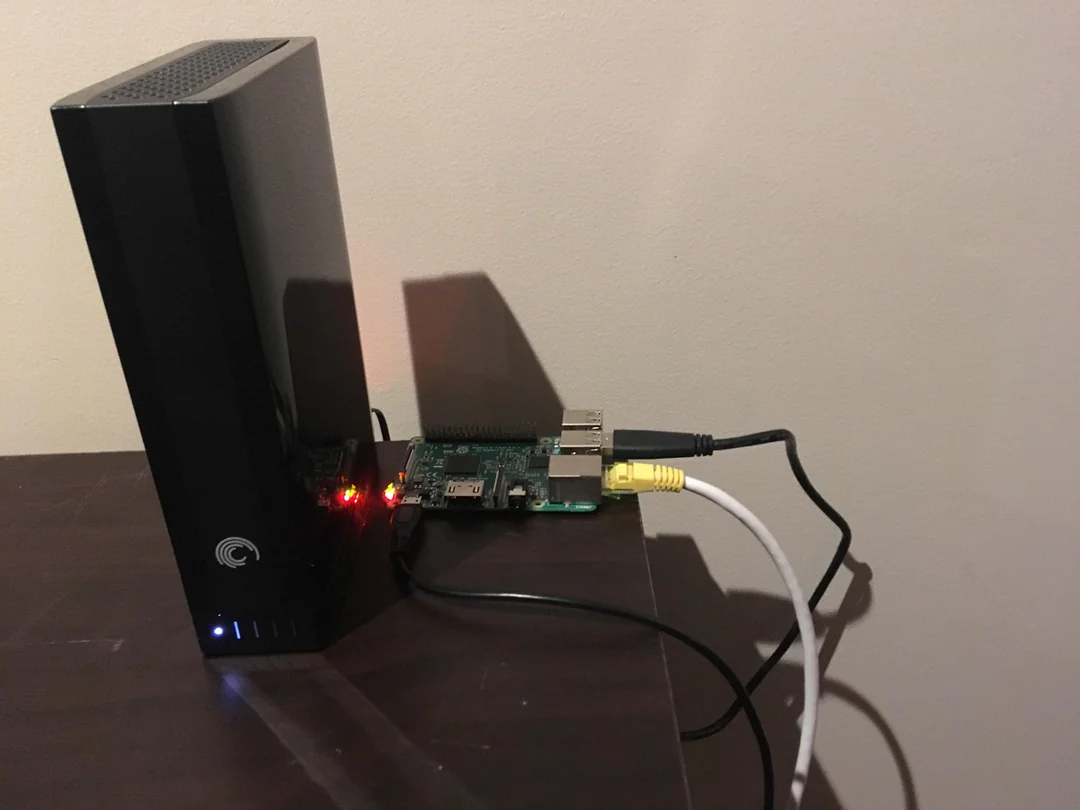
\includegraphics[height=.5\textheight]{budget-setup.png}
                    \caption{Budget-Homelab\\Quelle: \href{https://www.reddit.com/r/raspberry_pi/comments/9ck1aq/extremely_proud_of_my_first_project_a_basic_nas/}{Reddit}}
                    \label{fig:budget-homelab}
                \end{figure}
            \end{column}%
        \end{columns}
    \end{frame}

    \begin{frame}
        \slidehead{}
        \begin{columns}[T]
            \begin{column}{.5\textwidth}
                Beispiel: Even more Budget-Homelab
                \begin{itemize}
                    \item Alter Laptop (0€)
                \end{itemize}
            \end{column}%
            \begin{column}{.5\textwidth}
                \begin{figure}[ht!]
                    \centering
                    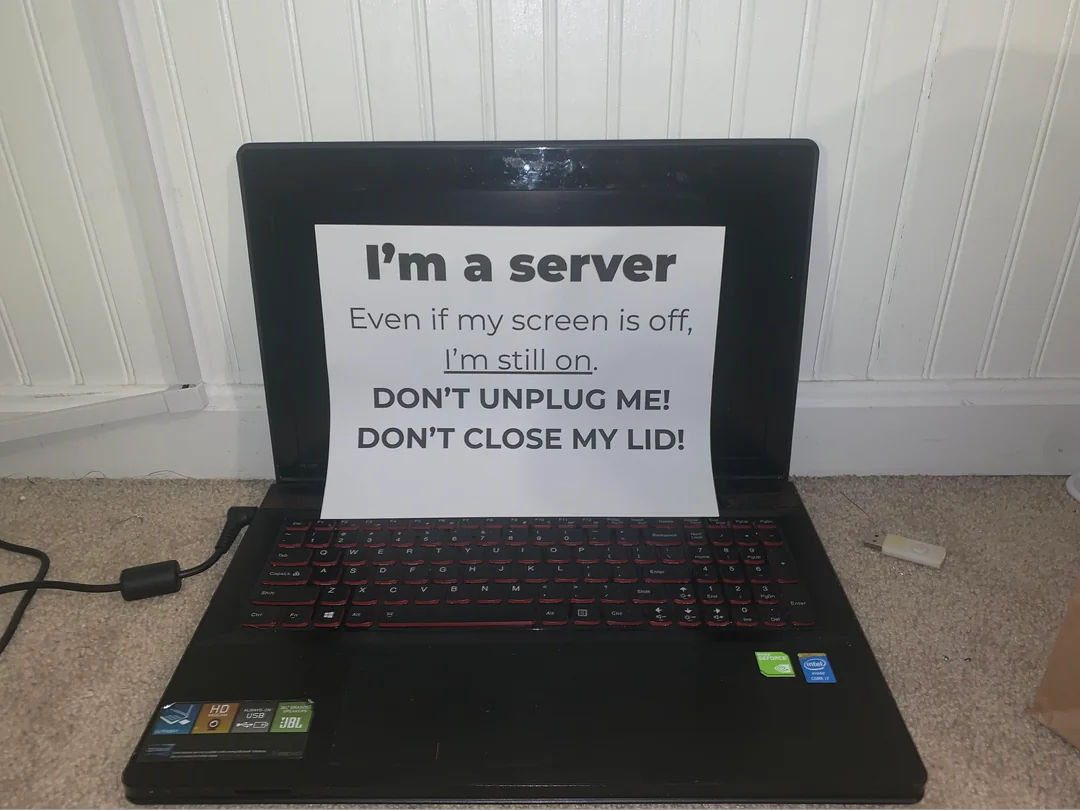
\includegraphics[height=.5\textheight]{even-more-budget-setup.png}
                    \caption{Even more Budget-Homelab\\Quelle: \href{https://www.reddit.com/r/ProgrammerHumor/comments/11u7tp7/linux_ideapad_server/}{Reddit}}
                    \label{fig:even-more-budget-homelab}
                \end{figure}
            \end{column}%
        \end{columns}
    \end{frame}

    \begin{frame}
        \slidehead{}
        \begin{columns}[T]
            \begin{column}{.5\textwidth}
                Beispiel: Average-Homelab
                \begin{itemize}
                    \item halbwegs okayer PC (ca. 500€+)
                    \item HDDs (ca. 20€/TB)
                    \item Gesamtkosten: ca. 700€+ (je nach Hardware)
                \end{itemize}
            \end{column}%
            \begin{column}{.5\textwidth}
                \begin{figure}[ht!]
                    \centering
                    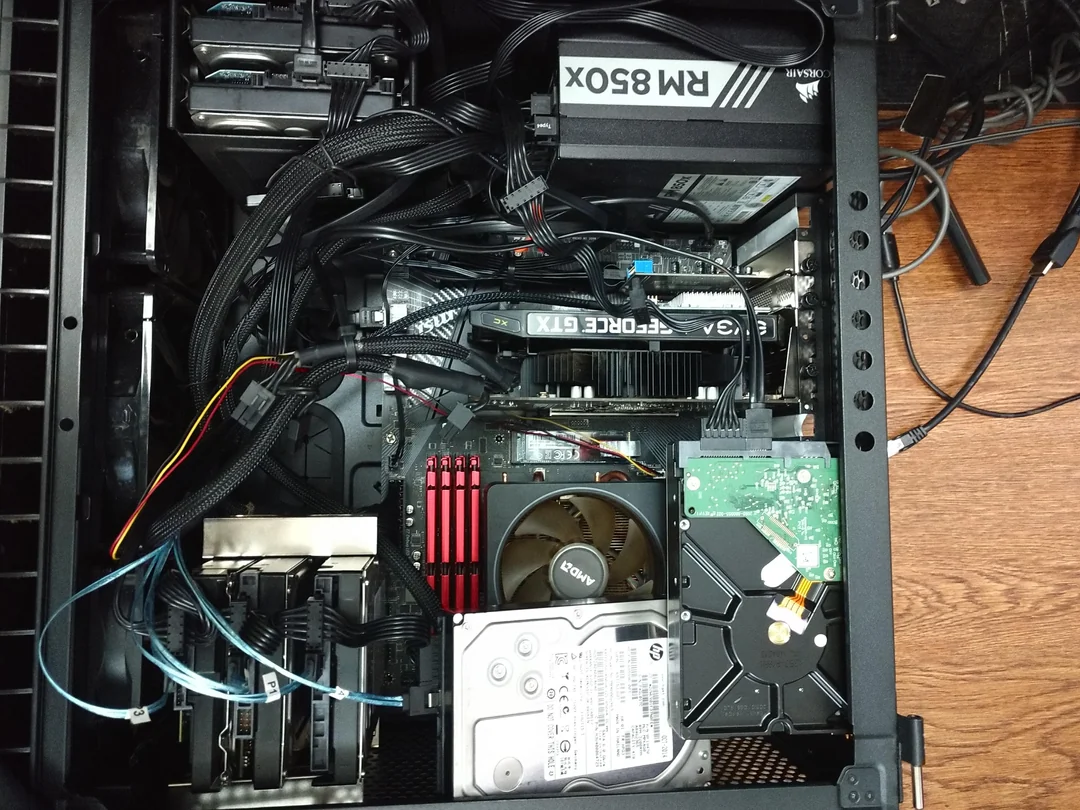
\includegraphics[height=.5\textheight]{average-setup.png}
                    \caption{Average-Homelab\\Quelle: \href{https://www.reddit.com/r/unRAID/comments/j6fcji/seven_35_hard_drives_in_a_mid_tower/}{Reddit}}
                    \label{fig:average-homelab}
                \end{figure}
            \end{column}%
        \end{columns}
    \end{frame}

    \begin{frame}
        \slidehead{}
        \begin{columns}[T]
            \begin{column}{.5\textwidth}
                Beispiel: Jetzt wirds ernst-Homelab
                \begin{itemize}
                    \item spezialisierte Hardware (ca. 1000€+)
                    \item HDDs/SSDs (ca. 20€/TB)
                    \item Redundanz (RAID, Backups, etc.)
                    \item spezielle Netzwerkgeräte, um Bandbreite voll auszunutzen (z.B. 10Gbit/s)
                    \item Gesamtkosten: so ca. 2000€+
                \end{itemize}
            \end{column}%
            \begin{column}{.5\textwidth}
                \begin{figure}[ht!]
                    \centering
                    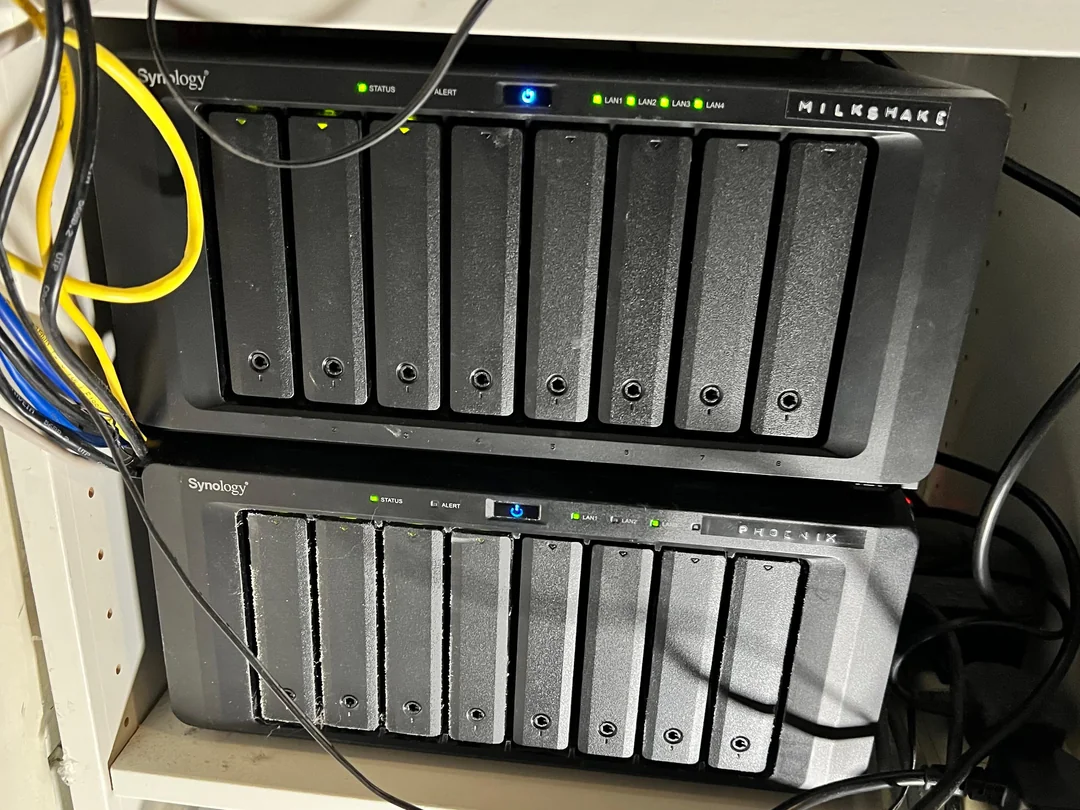
\includegraphics[height=.5\textheight]{jetzt-wirds-ernst-setup.png}
                    \caption{Jetzt wirds ernst\\Quelle: \href{https://www.reddit.com/r/synology/comments/10cxa9x/synology_networking_question_25gbe_on_the_cheap/}{Reddit}}
                    \label{fig:jetzt-wirds-ernst-homelab}
                \end{figure}
            \end{column}%
        \end{columns}
    \end{frame}

    \begin{frame}
        \slidehead{}
        \begin{columns}[T]
            \begin{column}{.5\textwidth}
                Beispiel: Ich hab zu viel Geld-Homelab
                \begin{itemize}
                    \item serverrack (ca. 10000€+)
                    \item RGB (macht alles schneller)
                    \item Cluster an Servern
                    \item Schallgedämmt
                    \item Macht mich neidisch
                \end{itemize}
            \end{column}%
            \begin{column}{.5\textwidth}
                \begin{figure}[ht!]
                    \centering
                    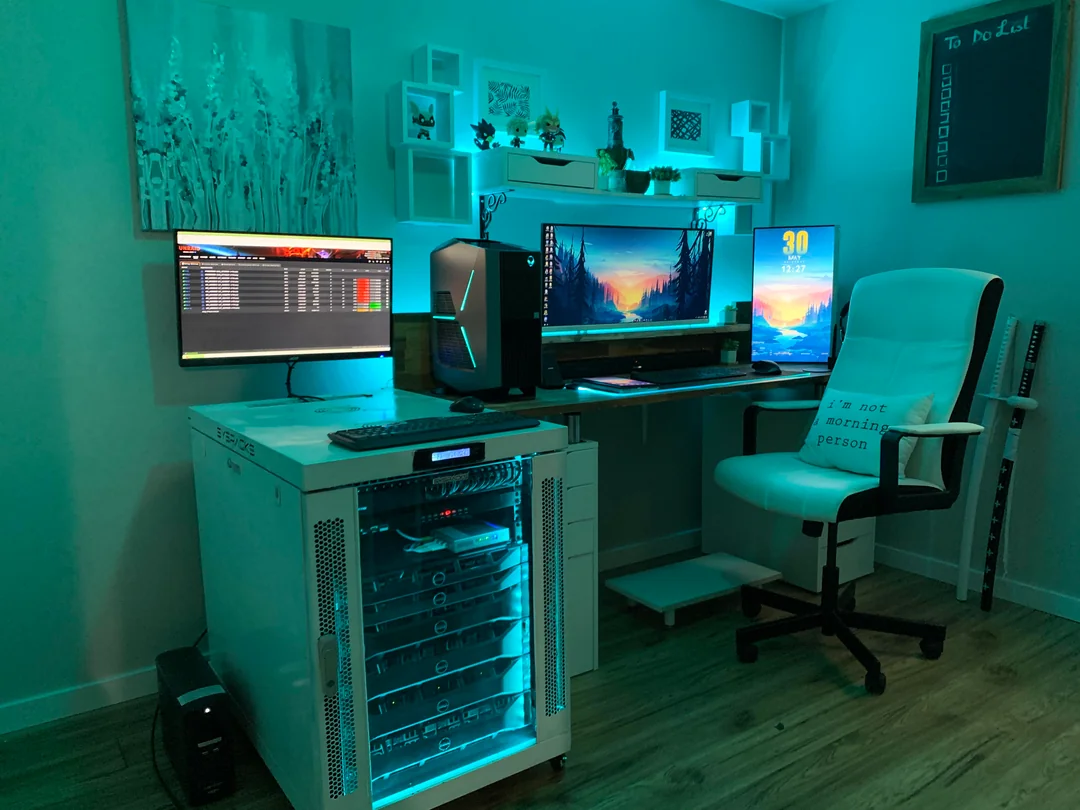
\includegraphics[height=.5\textheight]{ich-hab-zu-viel-geld-setup.png}
                    \caption{Ich hab zu viel Geld-Homelab-Homelab\\Quelle: \href{https://www.reddit.com/r/battlestations/comments/gtjihg/battlestation_meets_homelab/}{Reddit}}
                    \label{fig:ich-hab-zu-viel-geld-homelab}
                \end{figure}
            \end{column}%
        \end{columns}
    \end{frame}

    \begin{frame}
        \slidehead{}
        \begin{columns}[T]
            \begin{column}{.5\textwidth}
                Beispiel: Home-Datacenter
                \begin{itemize}
                    \item serverrack
                    \item 100Gbit/s Netzwerk
                    \item Glasfaseranbindung
                    \item Mehrere Server
                    \item SSDs (ca. 50€/TB)
                    \item Gesamtkosten: ca. 5000-6000€
                \end{itemize}
            \end{column}%
            \begin{column}{.5\textwidth}
                \begin{figure}[ht!]
                    \centering
                    \includegraphics[height=.5\textheight]{alex-setup.png}
                    \caption{Home-Datacenter\\Quelle: Alex}
                    \label{fig:home-datacenter}
                \end{figure}
            \end{column}%
        \end{columns}
    \end{frame}

    \begin{frame}
        \slidehead{}
        \begin{columns}[T]
            \begin{column}{.5\textwidth}
                Beispiel: WTF
                \begin{itemize}
                    \item mehrere Serverracks
                    \item 100Gbit/s Netzwerk
                    \item Mehrere Petabyte an Speicher
                    \item RGB (macht alles schneller)
                    \item GPU-Cluster
                    \item Gesamtkosten: $\infty$
                    \item Freundin? Die läuft auf Node-25
                \end{itemize}
            \end{column}%
            \begin{column}{.5\textwidth}
                \begin{figure}[ht!]
                    \centering
                    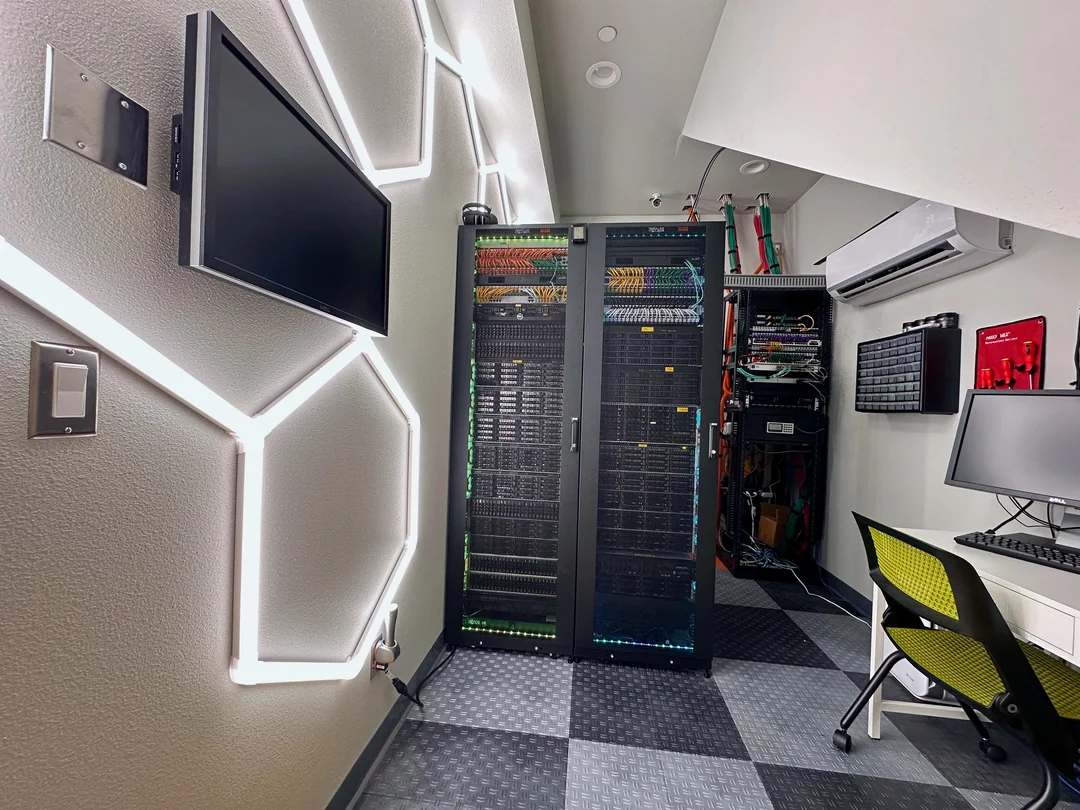
\includegraphics[height=.5\textheight]{wtf-homelab.png}
                    \caption{WTF\\Quelle: \href{https://www.reddit.com/r/homelab/comments/1bn3p75/the_never_ending_cable_cleanup_a_weekend_of/}{Reddit}}
                    \label{fig:wtf-homelab}
                \end{figure}
            \end{column}%
        \end{columns}
    \end{frame}

    \subsection{Was kann ich damit machen?}
    \begin{frame}
        \slidehead{}
        \vspace{-1em}
        \begin{columns}[c]
            \begin{column}{.5\textwidth}
                Self-Hosting
                \begin{itemize}
                    \item Weg von Cloud-Anbietern (Google, Amazon, Microsoft, etc.)
                        \begin{itemize}
                            \item Nextcloud statt Google Drive/Icloud
                            \item Collabora office statt Google Docs/Office 365
                            \item Jellyfin statt Netflix
                            \item Pihole als netzwerkweiter Adblocker
                            \item Home-Assistant für Smart-Home
                            \item OpnWRT statt FritzBox
                            \item Mycroft statt Alexa
                            \item etc.
                        \end{itemize}
                    \item Datenhoheit erlangen
                    \item experimentieren, lernen, Spaß haben
                \end{itemize}
            \end{column}%
            \begin{column}{.5\textwidth}
                \begin{figure}[ht!]
                    \centering
                    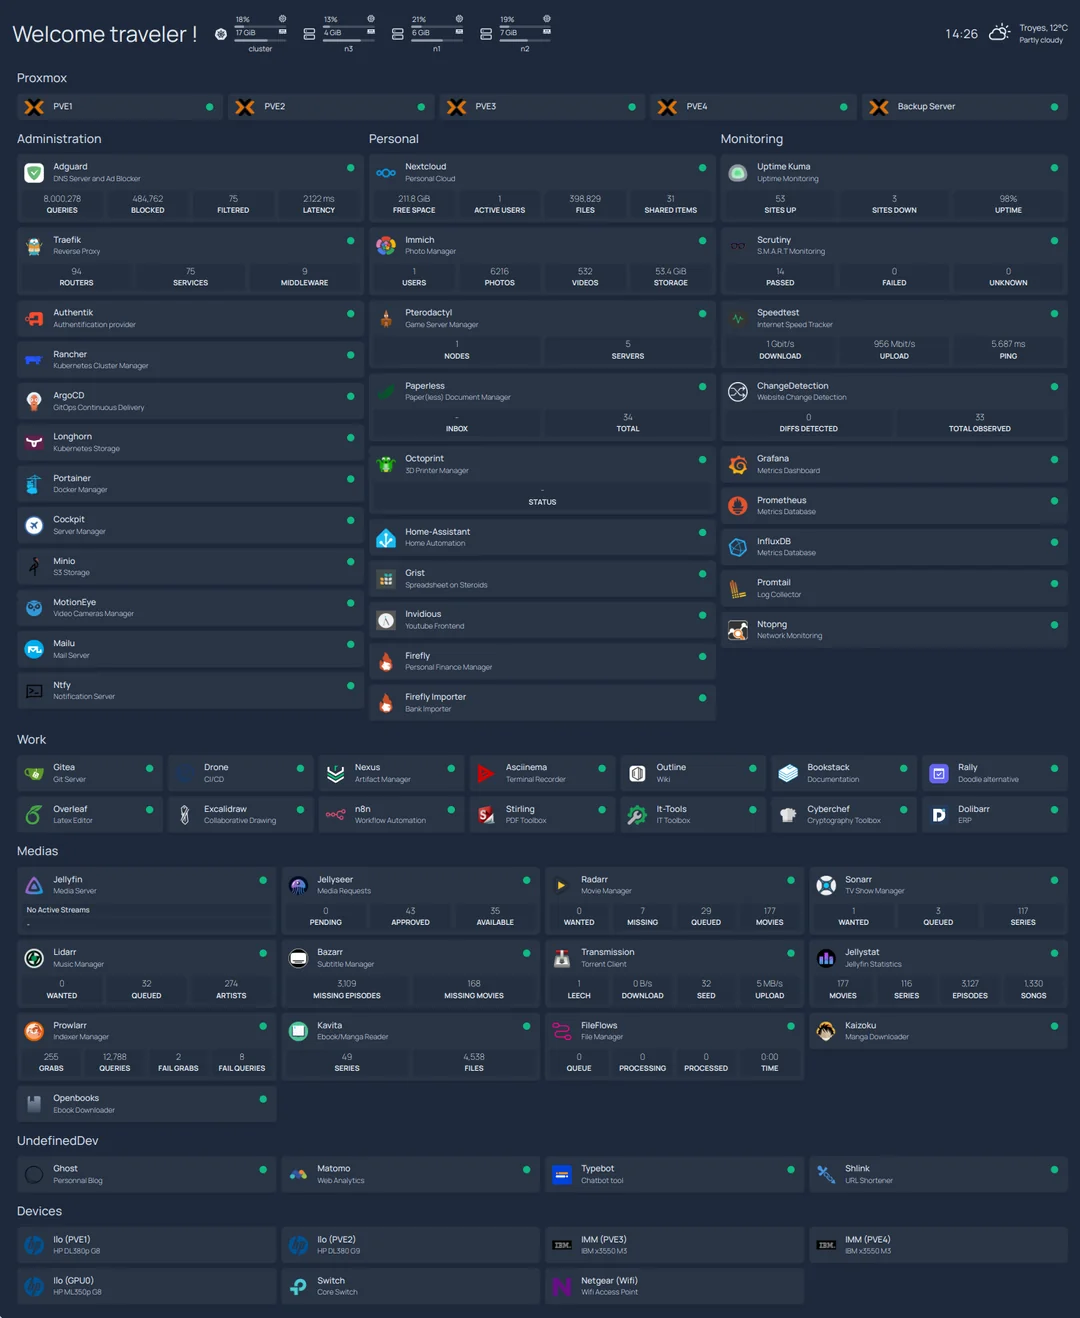
\includegraphics[height=.5\textheight]{self-hosting.png}
                    \caption{Homepage-Setup\\Quelle: \href{https://www.reddit.com/r/selfhosted/comments/18xgcsu/my_dashboard_now_with_descriptions/}{Reddit}}
                    \label{fig:self-hosting}

                \end{figure}
            \end{column}%
        \end{columns}
    \end{frame}

    \begin{frame}
        \slidehead{}
        \begin{columns}[T]
            \begin{column}{.5\textwidth}
                Smart-Home
                \begin{itemize}
                    \item meistens mit Home-Assistant
                    \item Autmatisierung/Fernsteuerung von:
                        \begin{itemize}
                            \item Licht (meist per Zigbee oder Z-Wave)
                            \item Heizung
                            \item Rasenmäher
                            \item etc.
                        \end{itemize}
                    \item Integration mit anderen Diensten (z.B. Mycroft, Alexa, etc.)
                \end{itemize}
            \end{column}%
            \begin{column}{.5\textwidth}
                \begin{figure}[ht!]
                    \centering
                    \includegraphics[height=.5\textheight]{home-assistant-rice.png}
                    \caption{Home-Assistant-Setup\\Quelle: \href{https://www.reddit.com/r/homeassistant/comments/1ftdstl/my_50_inches_family_dashoboard/}{Reddit}}
                    \label{fig:home-assistant}

                \end{figure}
            \end{column}%
        \end{columns}
    \end{frame}

    \begin{frame}
        \slidehead{}
        \begin{columns}
            \begin{column}{.5\textwidth}
                Basteln
                \begin{itemize}
                    \item Server, Netzwerkgeräte, etc. selbst zusammenbauen
                    \item Software selbst schreiben
                    \item Hardware modifizieren
                    \item Löten, 3D-Druck, etc.
                    \item Achtung: kann zum Vollzeitjob werden
                    \item Achtung: kann teuer werden
                \end{itemize}
            \end{column}%
            \begin{column}{.5\textwidth}
                \begin{figure}[ht!]
                    \centering
                    \includegraphics[height=.5\textheight]{basteln.png}
                    \caption{3D printed mini rack\\Quelle: \href{https://www.reddit.com/r/homelab/comments/lqr1gy/monty_3d_printed_mini_rack/}{Reddit}}
                    \label{fig:basteln}

                \end{figure}
            \end{column}%
        \end{columns}
    \end{frame}

    \begin{frame}
        \slidehead{}
        \begin{columns}
            \begin{column}{.5\textwidth}
                Kosten Sparen
                \begin{itemize}
                    \item Cloud-Speicher ist sehr teuer
                    \item Cloud-Computing ist sehr teuer
                    \item Daheim ist es billiger
                    \item Aber: \begin{itemize}
                            \item Hoher Zeitaufwand
                            \item Viel Verantwortung
                        \end{itemize}
                \end{itemize}
            \end{column}%
            \begin{column}{.5\textwidth}
                \begin{figure}[ht!]
                    \centering
                    \Huge\faDollarSign{}
                    \caption{Kosten Sparen}
                    \label{fig:kosten-sparen}
                \end{figure}
            \end{column}%
        \end{columns}
    \end{frame}
\end{document}
